%!TEX root = ../thesis.tex
%*******************************************************************************
%****************************** Second Chapter *********************************
%*******************************************************************************

\chapter{Simulation and Reconstruction}

The simulation of signal as well as background events is a critical part of the measurement
of the \ttbar cross section. The first step is the simulation of the result of the proton-proton 
collisions at a center of mass energy of $\sqrt{s} = 13 \; \TeV$. Then the decay and further interaction 
of the resulting particles is predicted. The final step is the simulation of the detector response.
Single events including all relevant particles and their kinematics are simulated.
The whole process is described in detail in Section \ref{sec:SimReco_Sim}.

In order to be analyzed, both the data and the simulation need to be reconstructed. The same algorithms are applied to ensure
that the simulation consistently models the data. 
The whole detector information is used to reconstruct particles and physics objects like electrons or jets.
The details can be found in Section \ref{sec:SimReco_Reco}. 


\section{Simulation}
\label{sec:SimReco_Sim}

The simulation of events involves multiple algorithms, most of which are shown in Figure \ref{fig:sim_struct}

\begin{figure}[htbp!]
  \begin{center}
      \resizebox{0.49 \textwidth}{!}{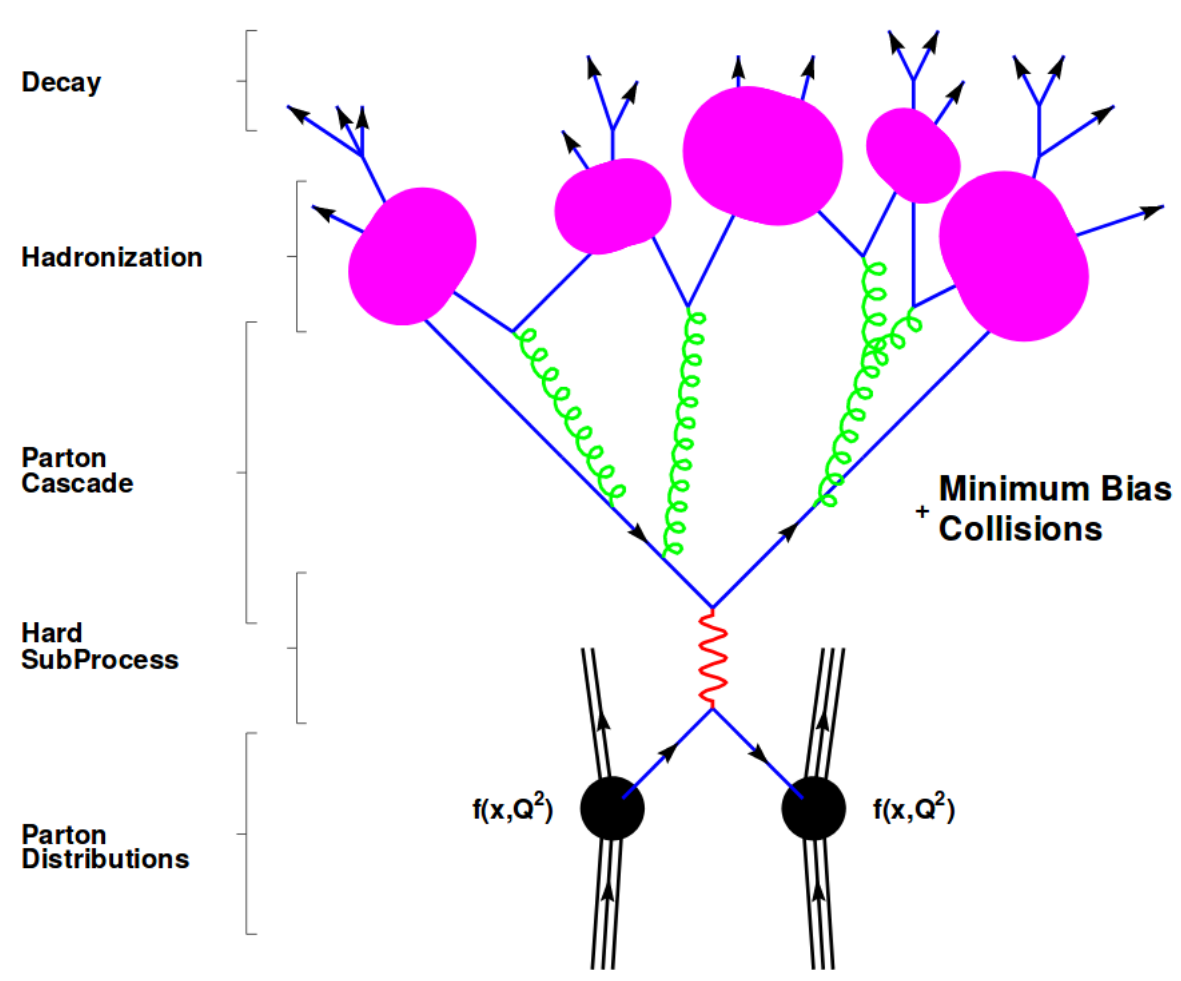
\includegraphics{SimReco/Figures/Event}}
\caption{Illustration of a simulated event split in multiple steps. Starting from the protons and the PDF continuing with the hard interaction, the parton shower, the hadronization and the decay of the hadrons\cite{Dobbs:684090}.
  \label{fig:sim_struct}}
  \end{center}
\end{figure}

The hard interaction for a given process like the production of \ttbar in proton-proton collisions is simulated by the matrix element generator.
This algorithm calculates the scattering amplitude of a given process and the kinematic properties of the resulting partons.
A large number of events is needed to avoid any bias due to the probabalistic nature of these distributions.
The interaction itself is calculated at a fixed order of QCD and can include additional radiation of quarks or gluons from the initial as well as the final state.
In the case of \ttbar events the matrix element generator also calculates the decay of the top quarks and the W bosons including the impact of spin correlations.

Since the particles in the initial state of the hard process are the constituents of the proton the probability to find a given constituent in a proton with a certain fraction of energy needs to be known.
This probability is given by Parton Distribution Functions(PDF) that predict the energy fraction of a given quark or gluon that is part of the proton.
In order to avoid singularities in the PDF calculation as well as in the hard interaction scales for the calculations of these divergences are introduced.
For the calculation of the proton substructure the factorization $\mu_F$ is used, while the scattering amplitude calculation uses the renormalization scale $\mu_R$.
The value of these scales are normally motivated by the mass of the heaviest particle involved in the process.
\todo{Needs some cites ?} 

Radiation beyond the scale of the matrix element generator is simulated by parton shower algorithms.
The radiation is calculated at a scale that can be set separately for initial and final state radiation. 
The parton shower algorithms generally follow phenomenological models and principally include QCD calculations up to all orders.
However, the parameters of these models are commonly tuned to match data from previous measurements.

As indicated by the name, the parton shower also simulates the showering of the partons that are the result of the hard process.
Especially quarks and gluons carrying a color charge contribute to further radiation forming hadronic showers.
These parton shower start from a maximum scale and evolve until a minimum scale on the order of \GeV. 

The combination of radiation of matrix element generator and parton shower can lead to double counting of radiation when the phase space overlaps.
This double counting can be minimised by using a matching procedure which varies according to the generator of parton shower that is used.

After the parton shower is cut off by the scale the resulting parton shower form color neutral hadrons.
This process is called hadronization and is part of the parton shower algorithm.
Again the hadronization is based on phenomenological methods whose settings have to be tuned.

The proton constituents not involved in the hard interaction are called proton remnants. The interaction of these proton remnants usually involve low energy processes and form the underlying
event (UE). The UE modelling is again tuned to data and included in the Parton Shower algorithm.

\begin{figure}[htbp!]
  \begin{center}
      \resizebox{0.49 \textwidth}{!}{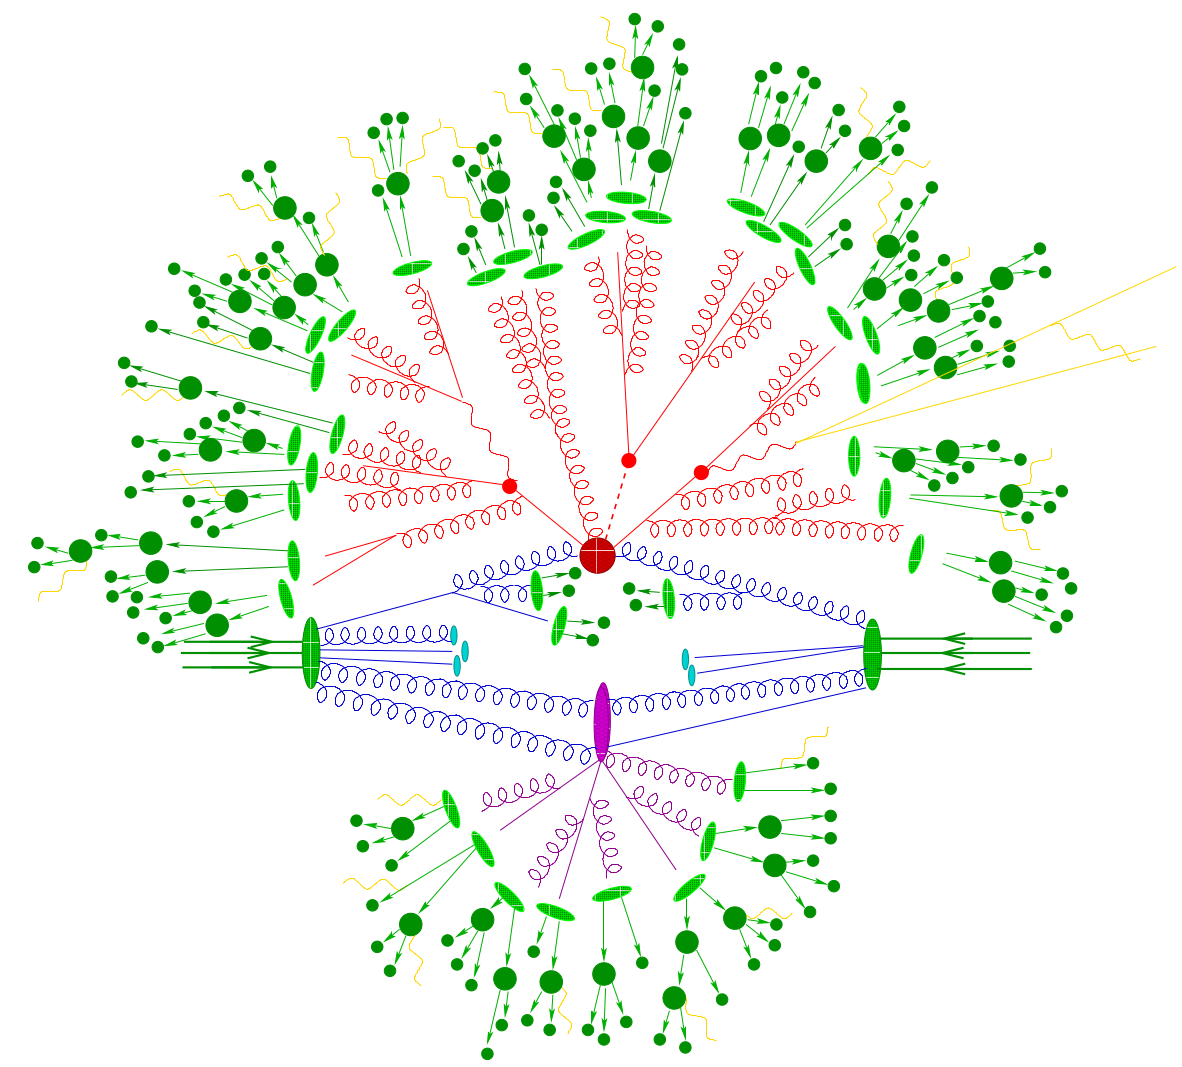
\includegraphics{SimReco/Figures/Sherpa}}
\caption{Representation of a simulated event from the Sherpa generator. It includes the hard interaction as well as showering, hadronization and underlying event\cite{Gleisberg:2008ta}.
  \label{fig:sim_sherpa}}
  \end{center}
\end{figure}

A whole event including the hard process and the Parton Shower is illustrated in Figure \ref{fig:sim_sherpa} showing the production of a top quark pair in association with a Higgs boson.
The incoming protons on the left and right sides are shownin the middle, with the blue gluons representing the initial state of the hard interaction.
The large red circle stands for the hard interaction with the initial state radiation shown in blue below.
The partons resulting from the hard interactions are shown above the hard process with smaller red circles. The final state radiation of gluons is also shown in red while additional radiation of photons is shown in orange.
The partons from the parton shower hadronize as illustrated by the green elipsi. The hadrons then decay into further hadrons.
Below the whole interaction, the underlying event is shown in violet.

The last part of the simulation is the modelling of the detector response which includes modelling the complete detector, simulating the interaction of particles with the detector material and the corresponding
response of the detector electronics. The full response of all detector subsystems including the trigger system is modelled for each event.

\subsection{Samples}
\todo{Title}

In this analysis the main generator is \Powheg~(v.~2)~\cite{bib:powheg2,Frixione:2007vw,Nason:2004rx} which calculates the production process at NLO. 
It is used for the simulation of the \ttbar signal as well as for most of the backgrounds.
The W+jets process is generated using \MGaMCatNLO~2.2.2~\cite{Alwall:2014hca,Frederix:2012ps} at NLO including up to two additional jets. The diboson background samples are generated with \Pythia~8.2~\cite{Sjostrand:2014zea}.
All samples are simulated with the NNPDF3.0~\cite{Ball:2012cx} PDF set.

\Pythia~8.2 is also used as parton shower algorithm for all samples. The CUETP8M2T4 tune~\cite{CMS-PAS-TOP-16-021,Skands:2014pea} used for the simulation of the signal.
The tuning is optimized for top physics by including \ttbar data taken with the CMS detector at a center of mass energy of $8 \TeV$.
For the backgrounds the standard tune for CMS CUETP8M1 tune is used.
\GEANT4 \cite{geant} is used to simulate the detector response for all samples.

The relevant cross sections for the relevant processes are taken from specific theory calculations as described in Chapter \todo{ref to Theory}.

\section{Reconstruction}
\label{sec:SimReco_Reco}

Different particles deposit energy in different parts of the detector as illustrated in Figure \ref{fig:reco_pflow}.
The tracks of charged particles are bent by the magnetic field, while neutral particles are unaffected.
Similarly only charged particles leave a signal in the tracker.
Electrons and photons deposit the main amount of their energy in the ECAL, whereas neutral and charged hadrons mainly deposit energy in the HCAL.
Muons are mainly detected by muon system in the outermost parts of the detector.
Phyics objects are reconstructed by combining this information from the basic elements of the detector using the Particle Flow algorithm \cite{Sirunyan:2017ulk}.

\begin{figure}[htbp!]
  \begin{center}
      \resizebox{0.80 \textwidth}{!}{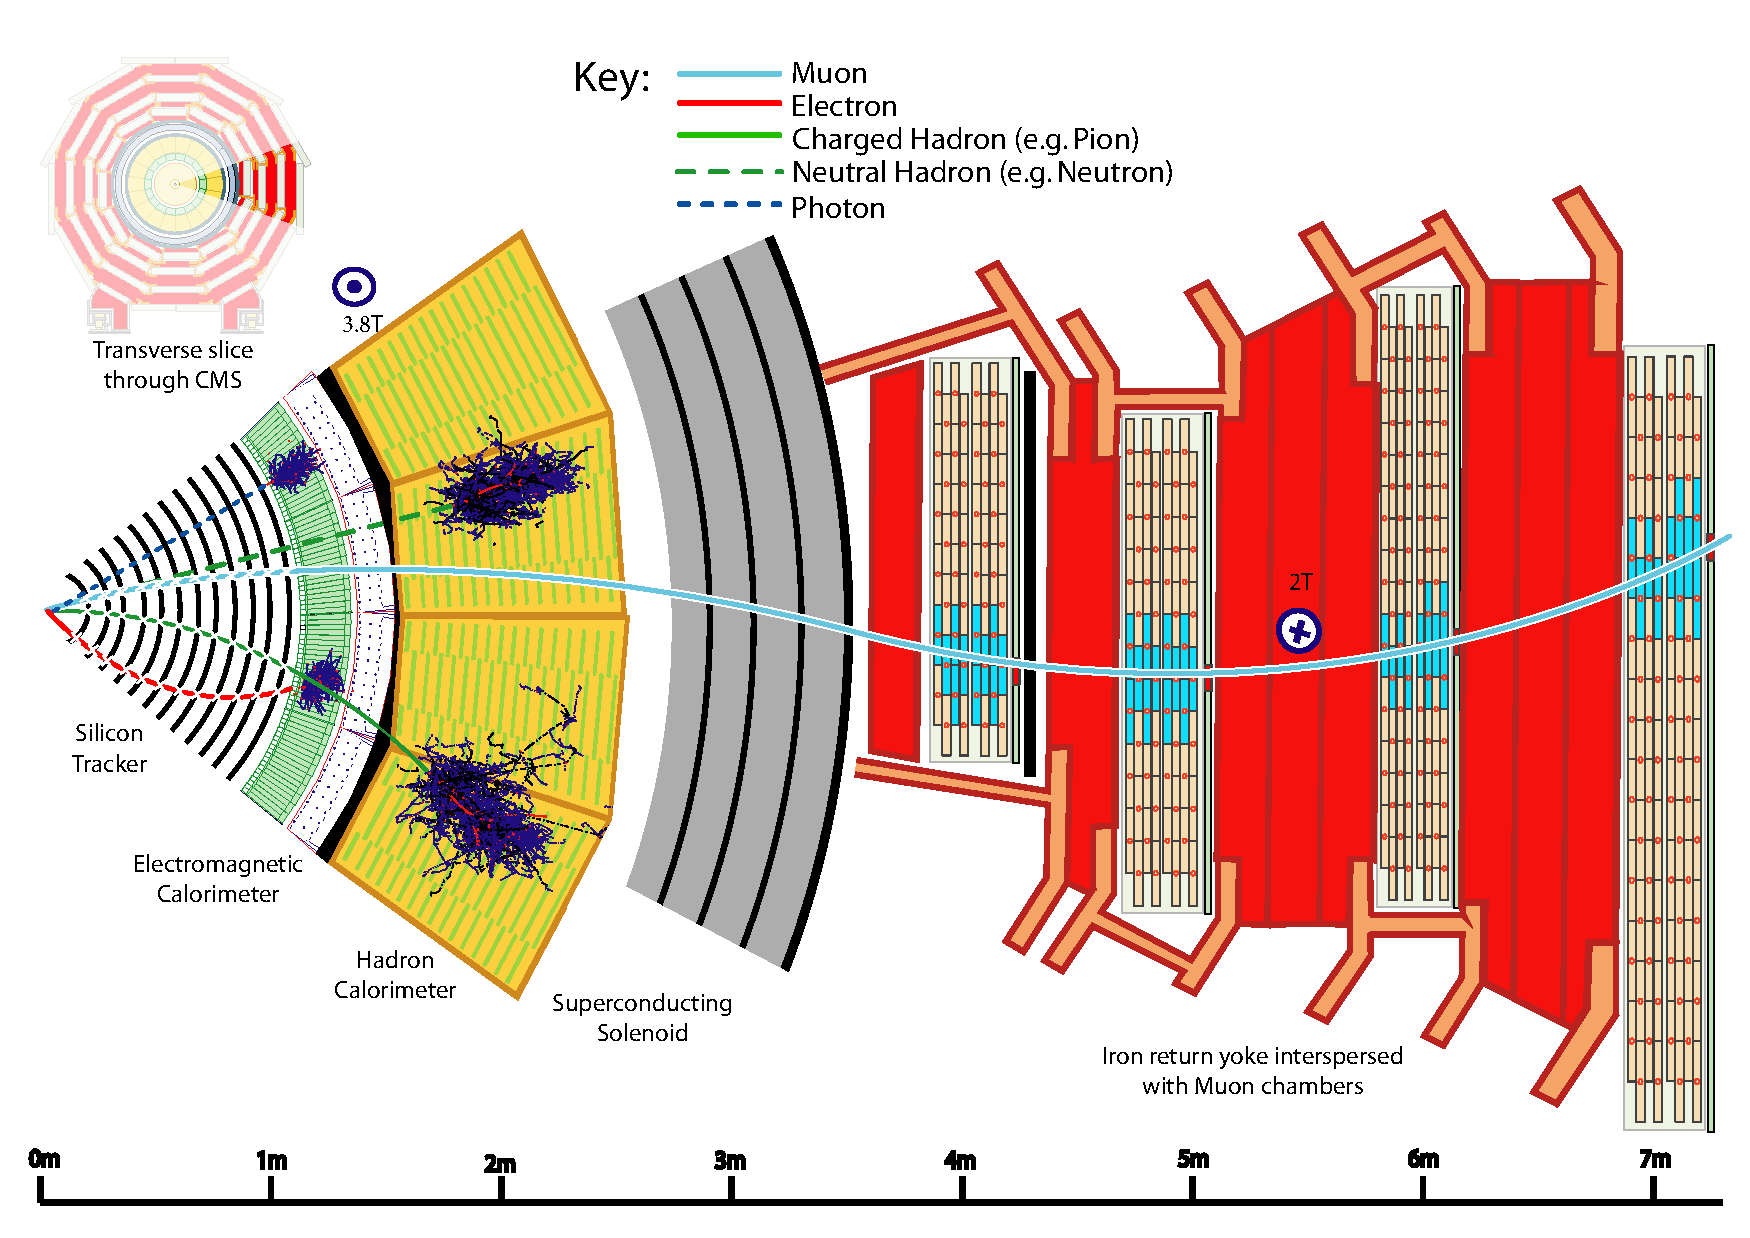
\includegraphics{SimReco/Figures/ParticleFlow.pdf}}
\caption{Illustration of the interaction of specific particles in a transverse slice of the CMS detector \cite{Sirunyan:2017ulk}.
  \label{fig:reco_pflow}}
  \end{center}
\end{figure}

In general, the probability to correctly reconstruct a particle can be different in simulation and measured data. Typically these differences are small, since the detector response
is modelled and the reconstruction algorithms for data and simulation are the same. Nevertheless, small differences remain, which are corrected in simulated events.
These corrections are typically defined separately for each physics object, by measuring the reconstruction efficiency independently in simulation and measured data.
The simulation is then corrected to fit the the efficiency measured in data. Resolution effects are corrected in a similar manner.

If all particles from a collision are correctly reconstructed the overall \pt of the events should be balanced, as the initial state particles do not have momentum in the transverse direction.
Particles that can not be reconstructed, such as neutrinos, lead to an imbalance in the overall transverse momenum called missing transverse energy, \ETmiss \cite{CMS-PAS-JME-16-004}.
The \ETmiss is reconstructed by a multi variate analysis using all other physics objects as well as unassociated energy deposits. It also takes the resolution of the other objects into account.
Since it is not used in the measurement, it is not described in further detail.


\subsection{Tracking and Vertex Reconstruction}

The aim of the tracking algorithm is to provide three properties of charged particles: The origin, the transverse momentum and the direction.
The track reconstruction itself is based on Kalman-Filtering \cite{Adam:934067} and consists of three steps starting with a seed of a few hits consistent with the trajectory of a charged particle.
The subsequent steps are the collection of hits from all tracker layers along the trajectory and the fitting to determin the aforementioned properties of the particle.
The tracking efficiency can be increased by repeating the track finding with different conditions.

The gain in efficiency through iterative tracking is presented in Figure \ref{fig:reco_trackingEff} showing the efficiency and the misreconstruction rate for tracks depending on the \pt of the charged particle for 
multiple different tracking algorithms. The efficiency is determined in simulation where tracks are considered to be reconstructed correctly if they are associated to a simulated particle. Correspondingly 
misreconstructed tracks are not associated to a simulated particle. 
Including all iterations shows a the highest efficiency and a comparative mistag rate. In general the efficiency decreases dramatically for high \pt tracks, especially for tracks with $\pt > 100 \gev$.
Similarly, the misreconstruction rate increases with higher \pt, but the effect can be mitigated when the rest of the detector is taken into account.

\begin{figure}[htbp!]
  \begin{center}
      \resizebox{0.49 \textwidth}{!}{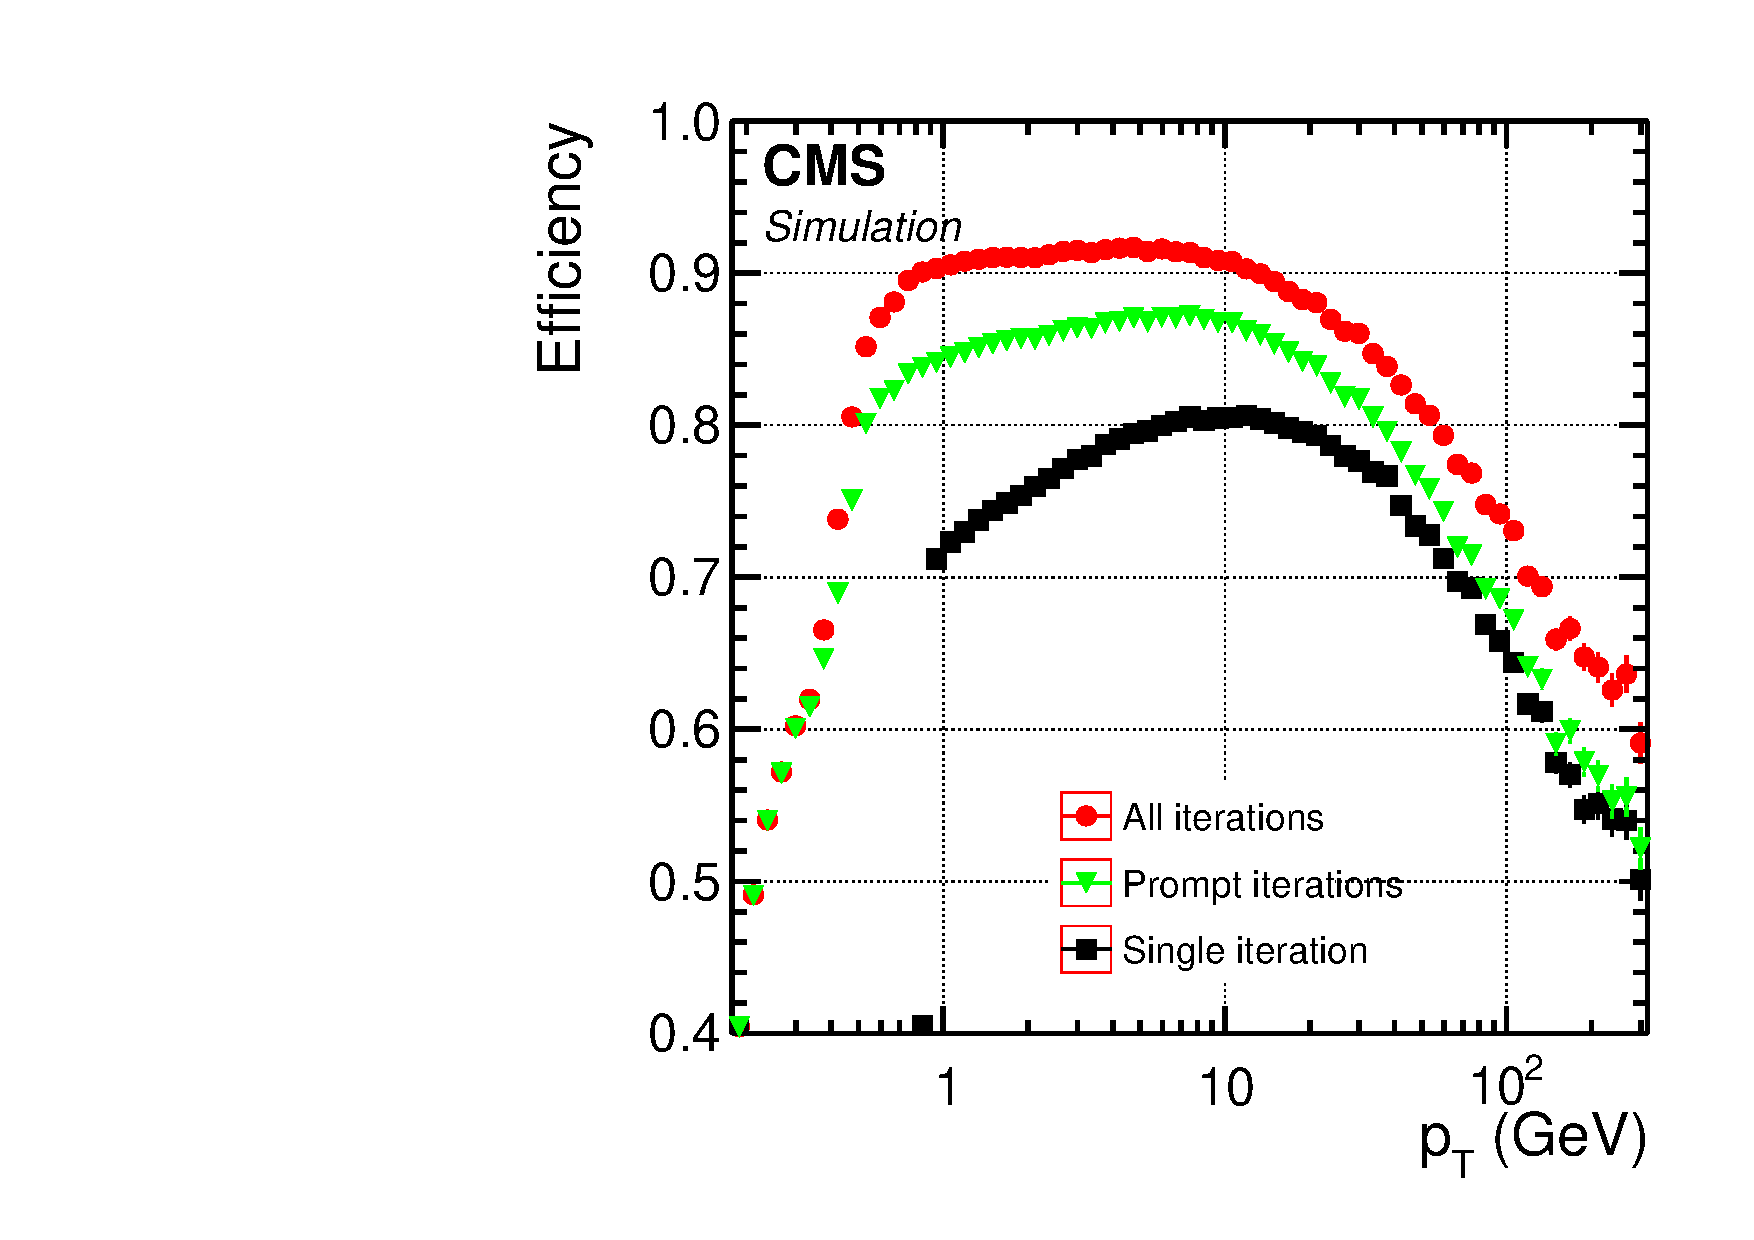
\includegraphics{SimReco/Figures/TrackingEff.pdf}}
      \resizebox{0.49 \textwidth}{!}{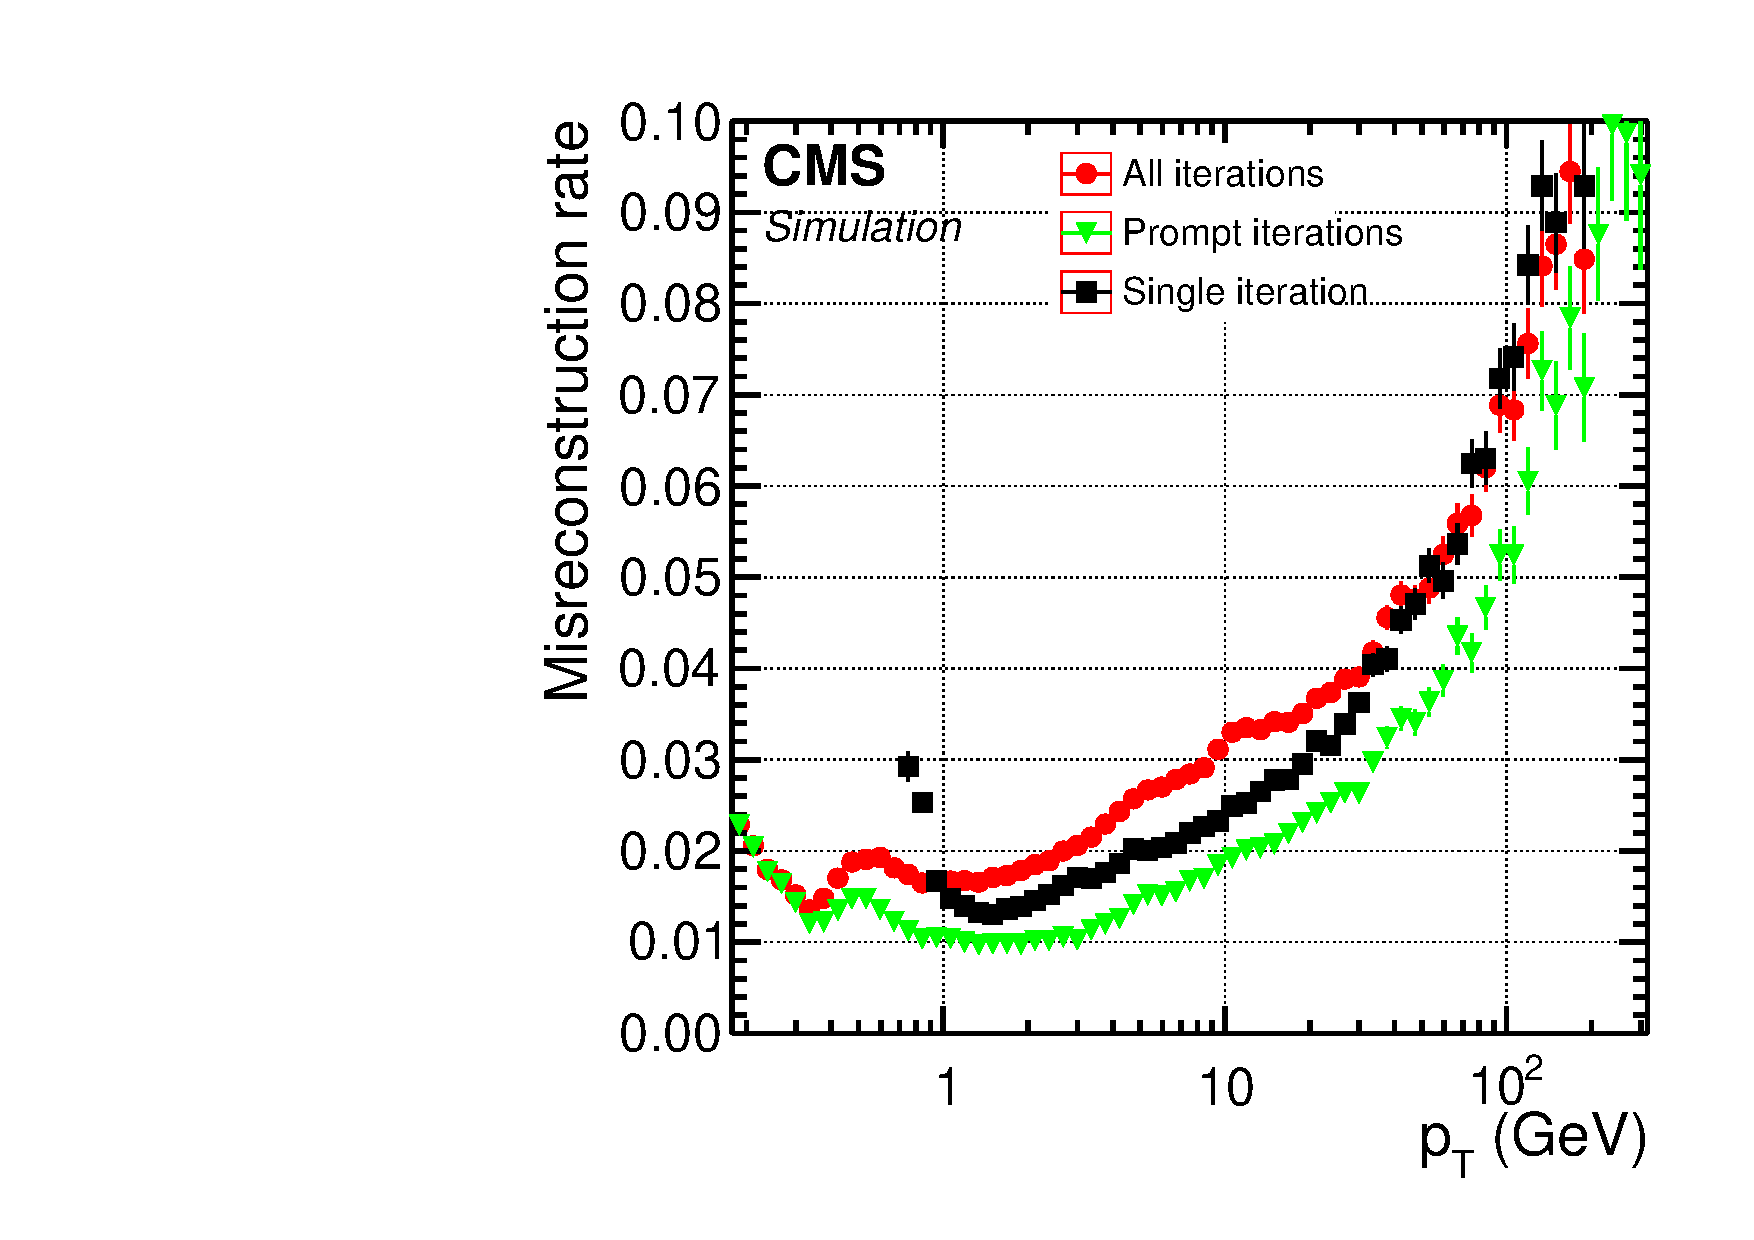
\includegraphics{SimReco/Figures/TrackingMis.pdf}}
\caption{Performance of the iterative tracking procedure\cite{Sirunyan:2017ulk}. The right plot shows the tracking efficiencies depending on the \pt of the charged particle for multiple different tracking approaches. 
         The left plot shows the rate to misreconstruct a track depending on the \pt of the charged particle for mutliple different tracking approaches. 
  \label{fig:reco_trackingEff}}
  \end{center}
\end{figure}

The origins of the tracks along the beam axis are considered as primary vertices and sorted according to the \pt of the associated tracks.
The vertex with the highest \pt is considered to be connected to the hard interaction. 
Additional vertices are caused by additional proton proton collisions occuring in the same bunch crossing as the hard interaction.
This so called pile-up leads to an average of 16 primary vertices in the 2016 dataset. It is mitigated by removing the contribution from
the pile-up vertices from the reconstruction.

\subsection{Electron Reconstruction}

The reconstruction of electrons is based on the combination of information from the tracker and the calorimeters.
The ECAL cluster containing the energy deposited by the electron and the related bremstrahlung is needed for both photon and electron reconstruction.
The corresponding HCAL region is required to have a only 10 \% of the energy deposited in the ECAL to avoid contamination with hadrons.
In order to be identified as an electron a particle needs a cluster of ECAL energy to be associated with a track.
In case no track is found the particle is identified as a photon.

The association between ECAL cluster and track can be either seeded from the tracker or from the ECAL.
In order to increase the efficiency both approaches are combined. The increase in efficiency from adding seeding from the tracker as determined in simulation is shown in Figure \ref{fig:reco_eletrackseed}.
The main gain of efficiency applies to electrons with a $\pt$ below 10 $\GeV$, but even electrons with higher \pt a few percent of efficiency is recovered.
Both the ECAL cluster and the track neeed to fullfill certain quality criteria applying to shower shape or track fitting.

\begin{figure}[htbp!]
  \begin{center}
      \resizebox{0.49 \textwidth}{!}{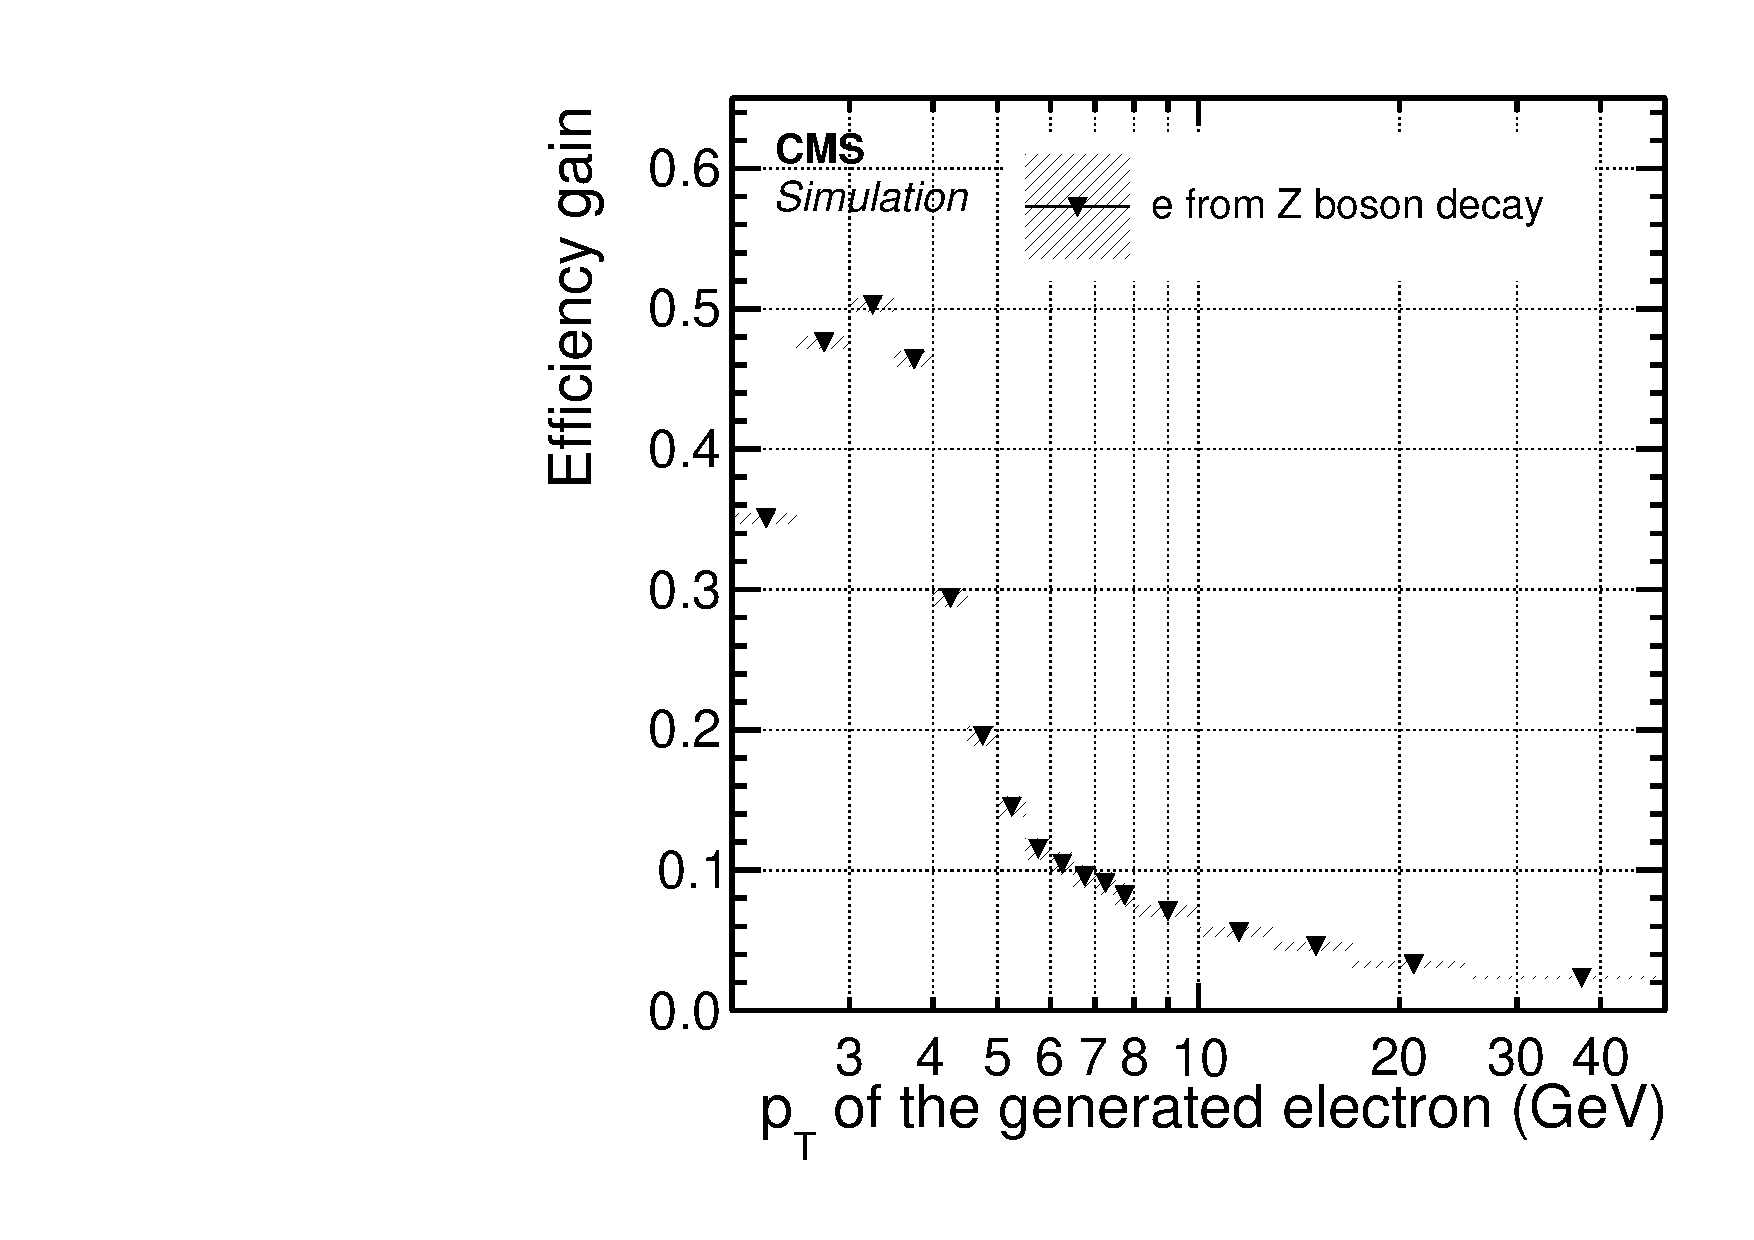
\includegraphics{SimReco/Figures/EleTrackSeed.pdf}}
\caption{Absolute gain in efficiency of the tracking in electrons when adding tracker-based seeding as a function of electron \pt\cite{Sirunyan:2017ulk}. 
         The efficiency is measured in simulated Z boson decays.
  \label{fig:reco_eletrackseed}}
  \end{center}
\end{figure}

Electrons are also required to be isolated: The energy deposited in a cone around an electron is required to be below 6 \% of the \pt of the electron.
The relative isolation is sensitive to contributions from pile-up. Contributions from charged particles that are not coming from the vertex of the hard collisions
are substracted from the isolation. The pile-up contributions from non-charged particles is harder to determin. It is estimated according to the general energy density
of the event and substracted from the isolation.
The combined efficiency to identify an electron is shown in Figure \ref{fig:reco_eleeff} depending on the \pt and the $\eta$ of the electron.
It is measured with the Tag and Probe method that is described in Section \ref{sec:TriggerTPMethod}.
The efficiency depends stronger on the $\pt$ of the electron than on its $\eta$ coordinate. The efficiency measured in data agrees with the one measured in simulation within $10\%$. 

\begin{figure}[htbp!]
  \begin{center}
      \resizebox{0.49 \textwidth}{!}{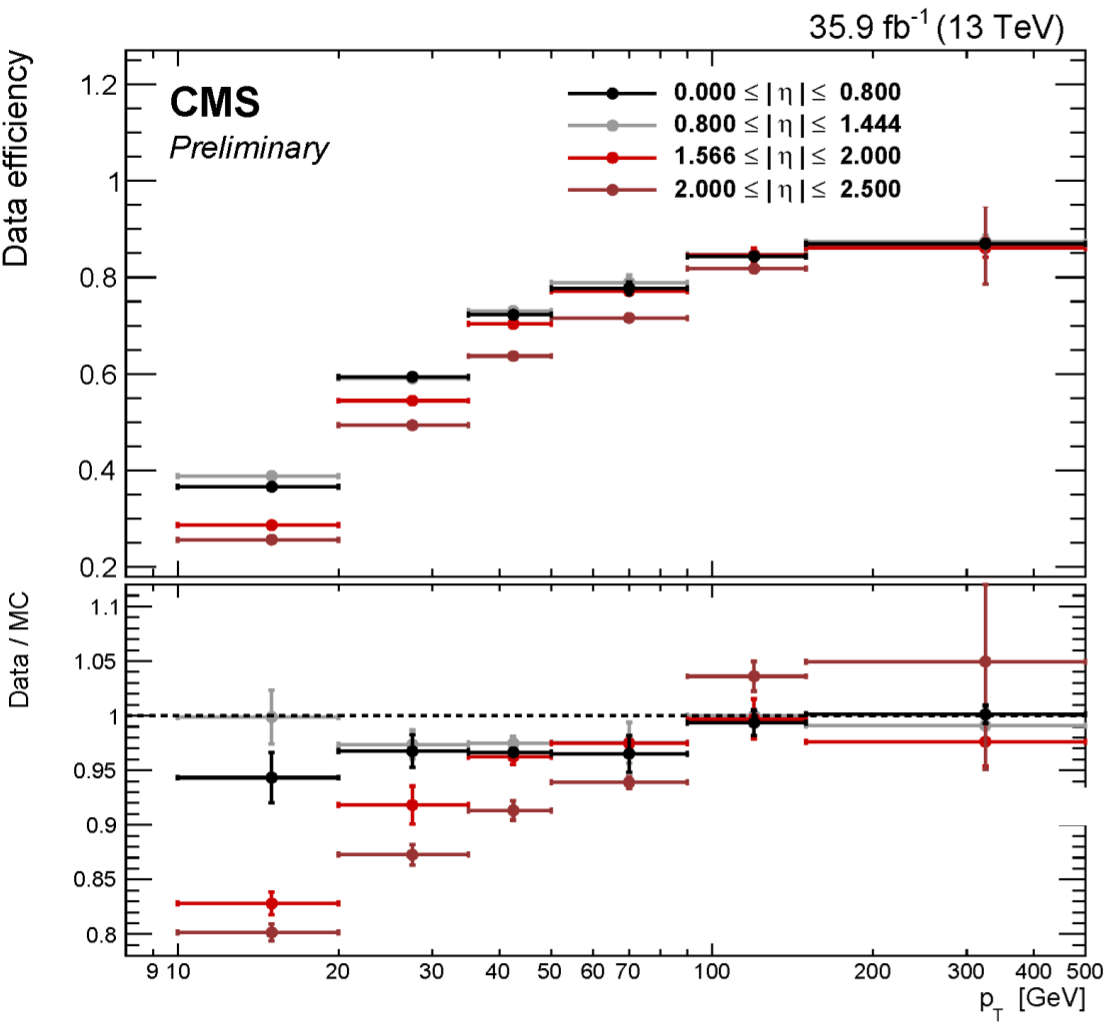
\includegraphics{SimReco/Figures/EleEff}}
\caption{Efficiency of the electron identification depending on the \pt and the $\eta$ of the electron\cite{CMS-DP-2017-004}.
         The upper pannel shows the efficiency measured in data. The lower pannel shows the efficiency in data divided by the efficiency in simulation. 
  \label{fig:reco_eleeff}}
  \end{center}
\end{figure}

The simulation is corrected according to the efficiency measurement in data. For each reconstructed electron a $\eta$ and \pt dependent weight is assigned to each event,
rescaling the simulation to match data. The weight itself is calculated by deviding the efficiency in data by the efficiency in simulation: $w = \epsilon_{\mathrm{data}} (\pt,\eta) /\epsilon_{\mathrm{MC}} (\pt,\eta)$.

The electron energy is corrected to cover known biases from the electromagnetic calorimeter. Additionally, the energy resolution is found to be higher in simulation when compared to data.
Both effects are visible when comparing the mass peak of the Z boson in events containing 2 electrons in data and simulation \ref{CMS-DP-2016-026}.
Since these events are well understood they allow to correct the disagreement by smearing the electron energy in simulation based on the $\eta$ and the shower shape of the electron.

\subsection{Muon Reconstruction}

Muons leave tracks in both the tracker and the muon system. For a reconstructed global the track in the muon system has to be matched to a track in the tracker.
The tracks need to be compatible with each other when propagated to a common surface.
Further quality requirements are applied to the inner track in the tracker.

Similar to the electrons, the muns are also required to be isolated. The energy deposited in a cone around the muon (isolation) is required to be below 15 \% of the muon \pt.
This energy has to originate from charged particles coming from the primary vertex, neutral hadrons or photons. The impact of the pile-up on the neutral hadron and photon components
is estimated to be half of the contribution from charged pile-up and is substracted from the total isolation.
The efficiency (measured with the Tag and Probe method, see Section \ref{sec:TriggerTPMethod}) for the identification and isolation requirements used in the analysis is shown in Figure \ref{fig:reco_mueff}.
The efficiency is above $90\%$ over nearly the whole range of $\eta$ and $\pt$.


\begin{figure}[htbp!]
  \begin{center}
      \resizebox{0.49 \textwidth}{!}{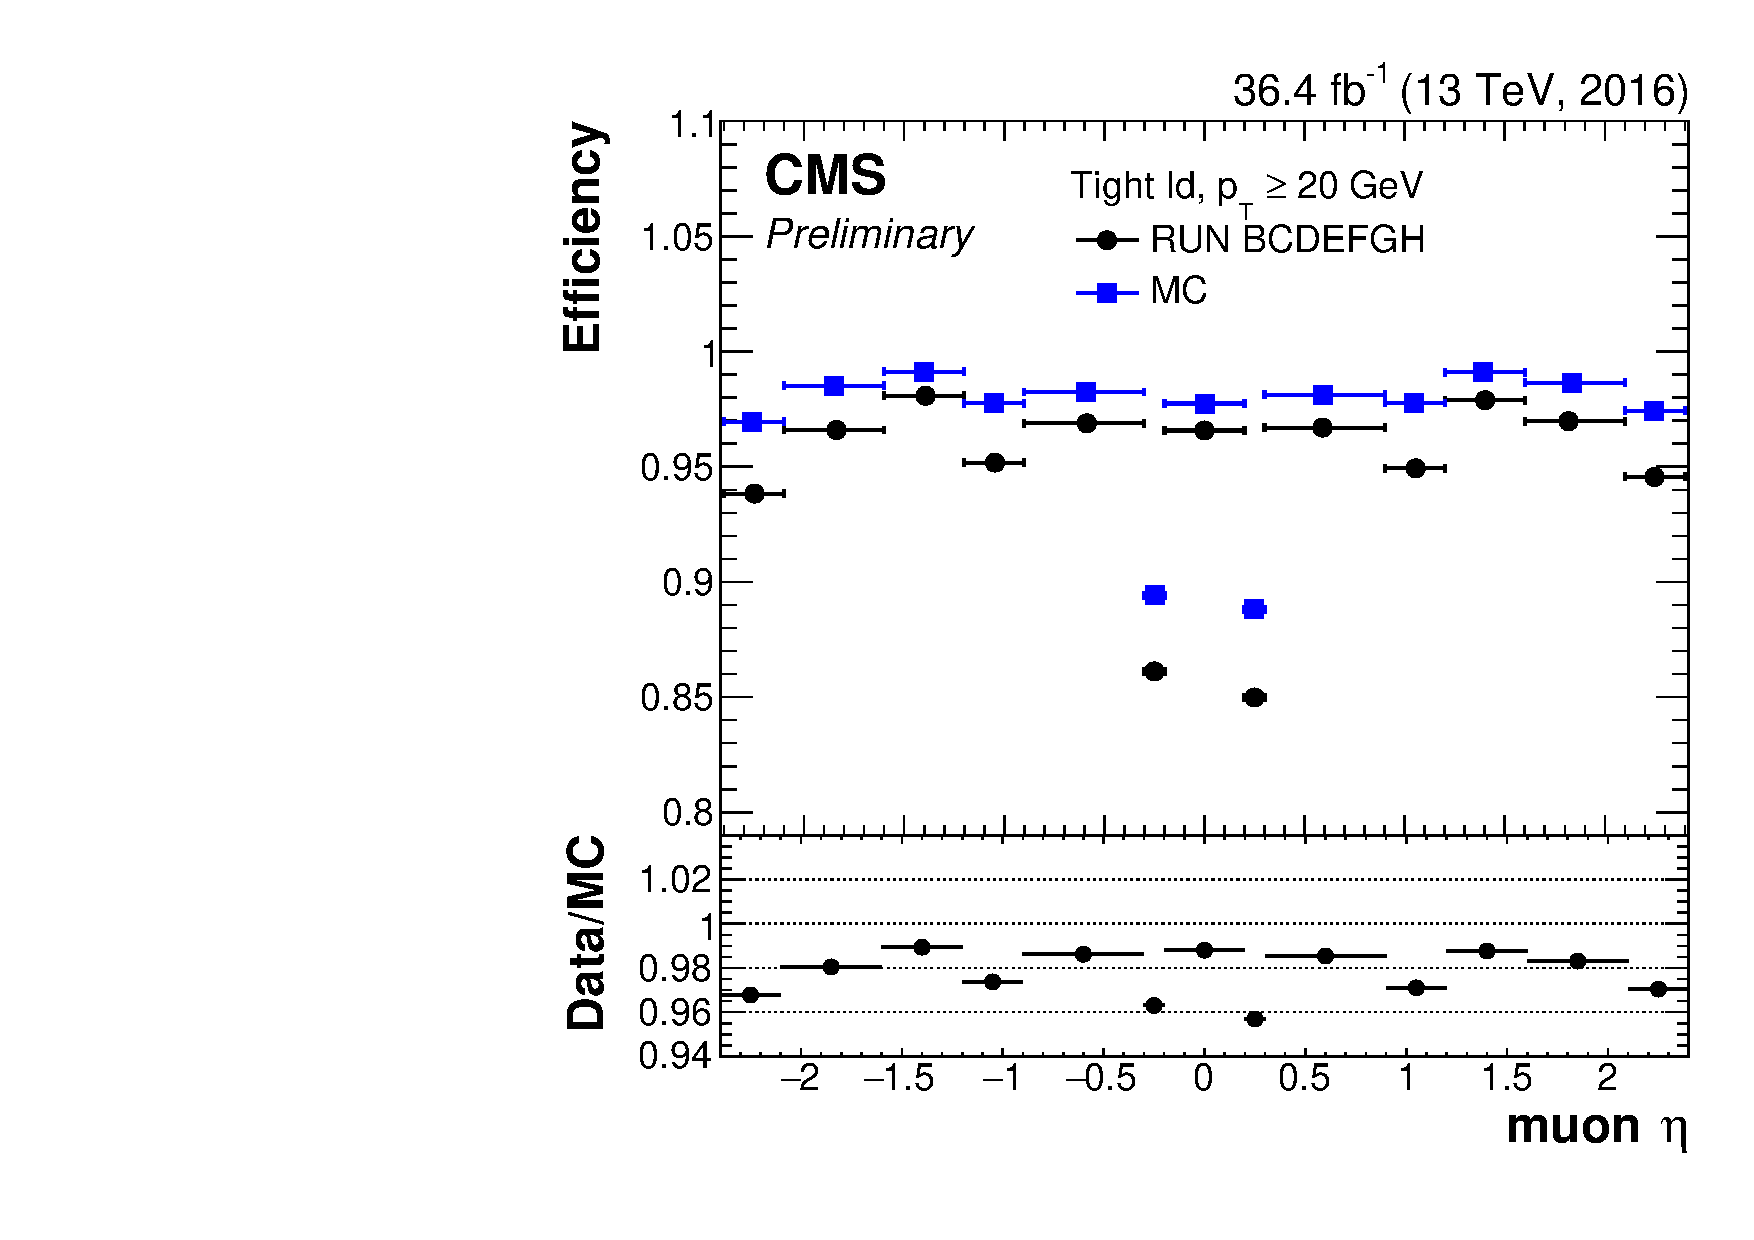
\includegraphics{SimReco/Figures/MuonIDEff}}
      \resizebox{0.49 \textwidth}{!}{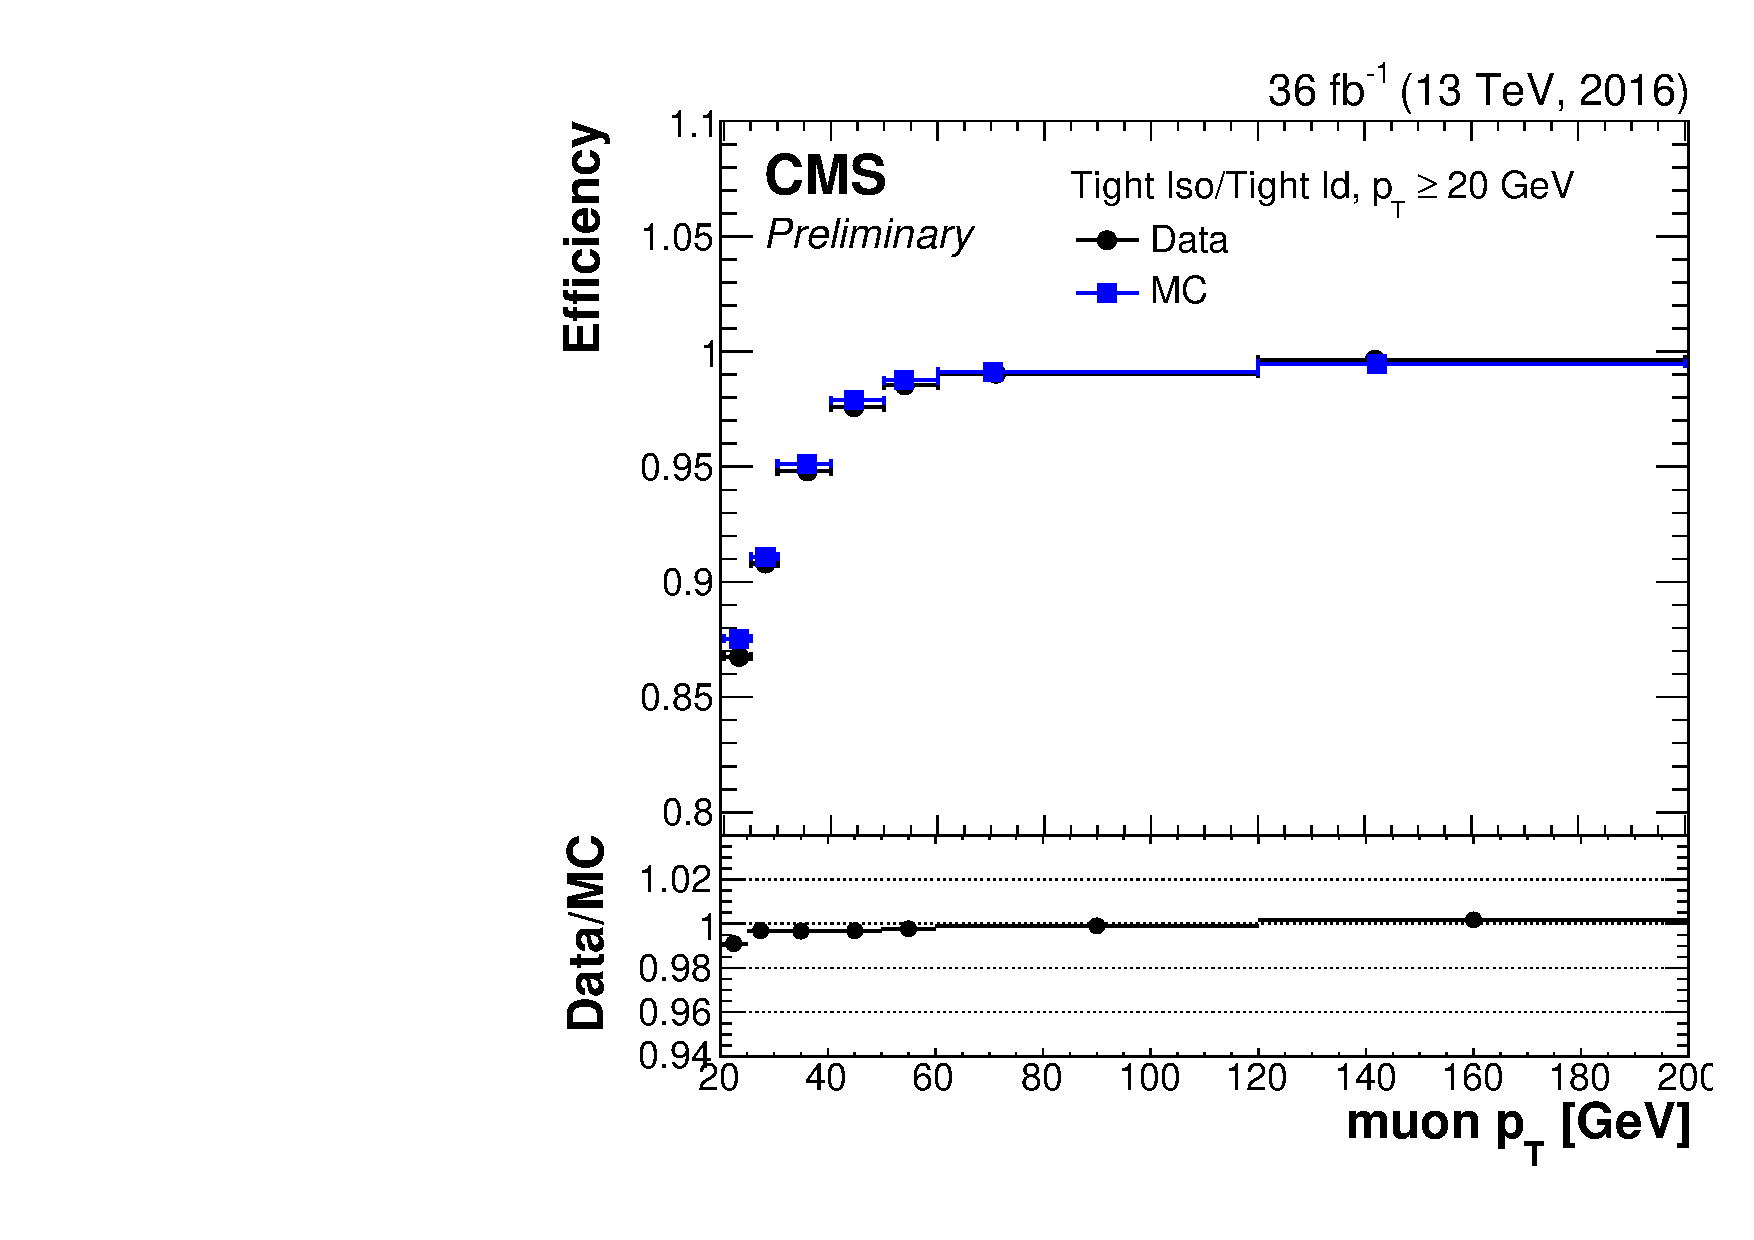
\includegraphics{SimReco/Figures/MuonIsoEff}}    
\caption{Efficiency of the identification (left) and isolation (right) for muons depending on $\eta$ (left) and $\pt$ right of the muon.
         The upper pannels show the efficiency in data and simulation, while the lower pannels show the ratio.
  \label{fig:reco_mueff}}
  \end{center}
\end{figure}

As described above for electrons, the mismatch in the efficiency in data and simulation is corrected by reweighting events.

The resolution and scale of the \pt of the muons in data and simulation can be investigated by comparing the mass peak of the Z boson depending on the $\eta$ and $\phi$ of the two leptons.
Additionally, the forward and backward charge assymetry is sensitive to differences between data and simulation.
The \pt of the muons is then corrected in simulation according to the disagreement observed. The corrections depend on the kinematics of the muon, its charge, the properties of the track of the muon and the simulated \pt
of the muon before the detector simulation.

\subsection{Reconstruction of Jets}
\label{sec:SimReco_BjetReco}

Jets are clustered from the individual particles reconstructed from the particle flow algorithm \cite{CMS-PAS-JME-16-003}.
The clustering uses the anti-\kt algorithm \cite{Cacciari:2008gp} as implemented in \FASTJET \cite{Cacciari:2011ma} with a distance parameter of $R = 0.4$.
The impact of pile-iup is reduced by removing charged hadrons not originating from the primary vertex from the particles that are clustered \cite{CMS-PAS-JME-14-001}.
Neutral particles originating from pile-up are taken into account by correcting the jet 4-momenta for each event based on the jet area \cite{1126-6708-2008-04-005,CACCIARI2008119}.

\begin{figure}[htbp!]
  \begin{center}
      \resizebox{0.89 \textwidth}{!}{
\includegraphics{SimReco/Figures/JECDiagram}}  
\caption{Illustration of the sequential jet energy scale corrections applied to measured data and simulation \cite{Khachatryan:2016kdb}. The flavor correction is not applied.
  \label{fig:reco_jec}}
  \end{center}
\end{figure}


The corrections for the jet energy scale are illustrated in Figure \ref{fig:reco_JEC}. They are applied sequentially to both measured data and simulation \cite{Khachatryan:2016kdb,CMS-PAS-JME-16-003}.
The first step corrects for remaining contributions from pile-up, which are determined by comparing jets in simulated events with and without the simulation of additional pile-up collisions.
In data an additional correction is derived from the Random Cone method in zero bias events. The correction is paramertrized depending on the energy density in the event, the jet are and the kinematic
properties of the jet. The pile-up correction also depends on the data taking period.

In the next step the reconstructed jet energy in simulation is compared to the energy of a simulated jet before the detector simulation (explicitly excluding neutrinos).
The correction is applied to both measured data and simulation and the reconstruction and depends on the \pt and $\eta$ of the jets.

The last correction is only applied to data, since flavor corrections are not used. It corrects for remaining differences in the jet response between data and simulation, which are determined
from dijet events. The correction depends on the \pt and $\eta$ of the jets.

The different jet response in measured data and simulation is illustrated in Figure \ref{fig:reco_jetresponse} showing the response measured in events containing photons and jets, and Drell-Yan events.
It also shows the uncertainty of the jet energy scale corrections. The numbers shown here are derived only for a subset of the full dataset and do not correspond to the corrections used later in the measurement.

\begin{figure}[htbp!]
  \begin{center}
      \resizebox{0.49 \textwidth}{!}{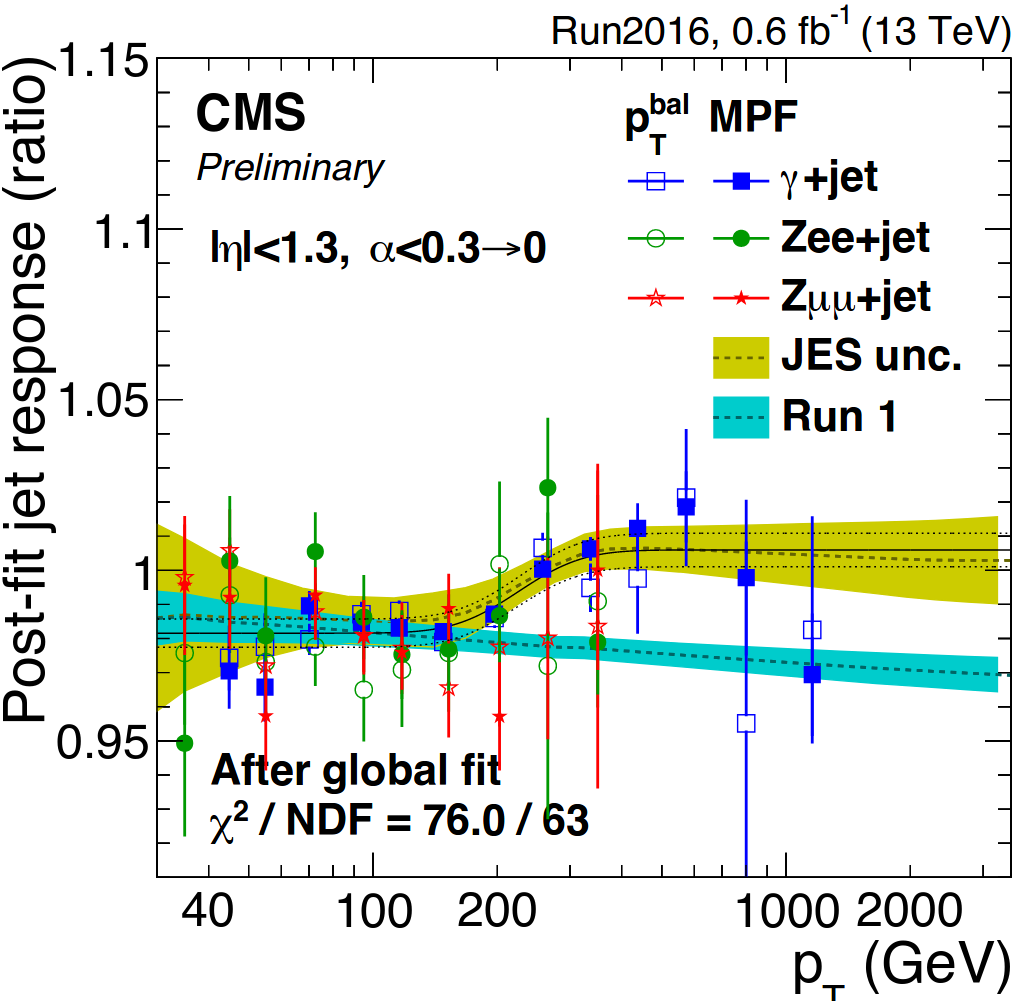
\includegraphics{SimReco/Figures/JetResponse}}  
\caption{The data to simulation ratio of the jet response measured in photon + jets and Z + jets events for a subset of data \cite{CMS-DP-2016-020}. The uncertainty for this dataset as well as the uncertainty for the dataset taken by the CMS collaboration
in Run 1 of the LHC are shown as colored bands. 
  \label{fig:reco_jetresponse}}
  \end{center}
\end{figure}


The jet energy resolution is determined from the width of the jet response function. It is found to be different in measured data and simulation. The \pt of the jets in simulation is rescaled depending on the simulation by the following
factor:

\begin{equation}
SF = 1 + (SF_{\mathrm{reso.}}-1) \frac{\pt - \pt^{gen}}{\pt}.
\end{equation}
Here, $SF_{\mathrm{reso.}}$ denotes the resolution scale factor and $\pt^{gen}$ stands for the \pt of the simulated jet before the simulation of the detector response. 

\subsection{Identification of b-Jets}

The large lifetime of the B Hadron leads to a decay that is often displaced from the original interaction.
These secondary vertices together with the displaced tracks and the properties of the jet itself are combined in the CSVv2 algorithm to identify jets originating from a b quark \cite{BTV16002}.
Sensitive variables are combined into a neural network which is trained against both jets originating from light jets as well as jets originating from c quarks.
The result is a single value (discriminator) with the cut chosen according to the desired efficiency and background rejection.

The tight working point chosen for this analysis has a very low rate of misidentifying a light jet as a b jet (mistag rate) with $\sim 0.1\%$. The efficiency to correctly identify a jet from a b quark
as a b jet is measured to be $\sim 40 \%$ \cite{BTV16002}. These numbers are obtained for jets with an average transverse momentum of $\pt = 70\;\GeV$. A lower efficiency can be expected for b jets with a lower \pt.

The efficiency in simulation is corrected according to the efficiency measured in data. The difference measured in events containing both muons and jets and in \ttbar events is shown in Figure \ref{fig:reco_btagsf}.

\begin{figure}[htbp!]
  \begin{center}
      \resizebox{0.89 \textwidth}{!}{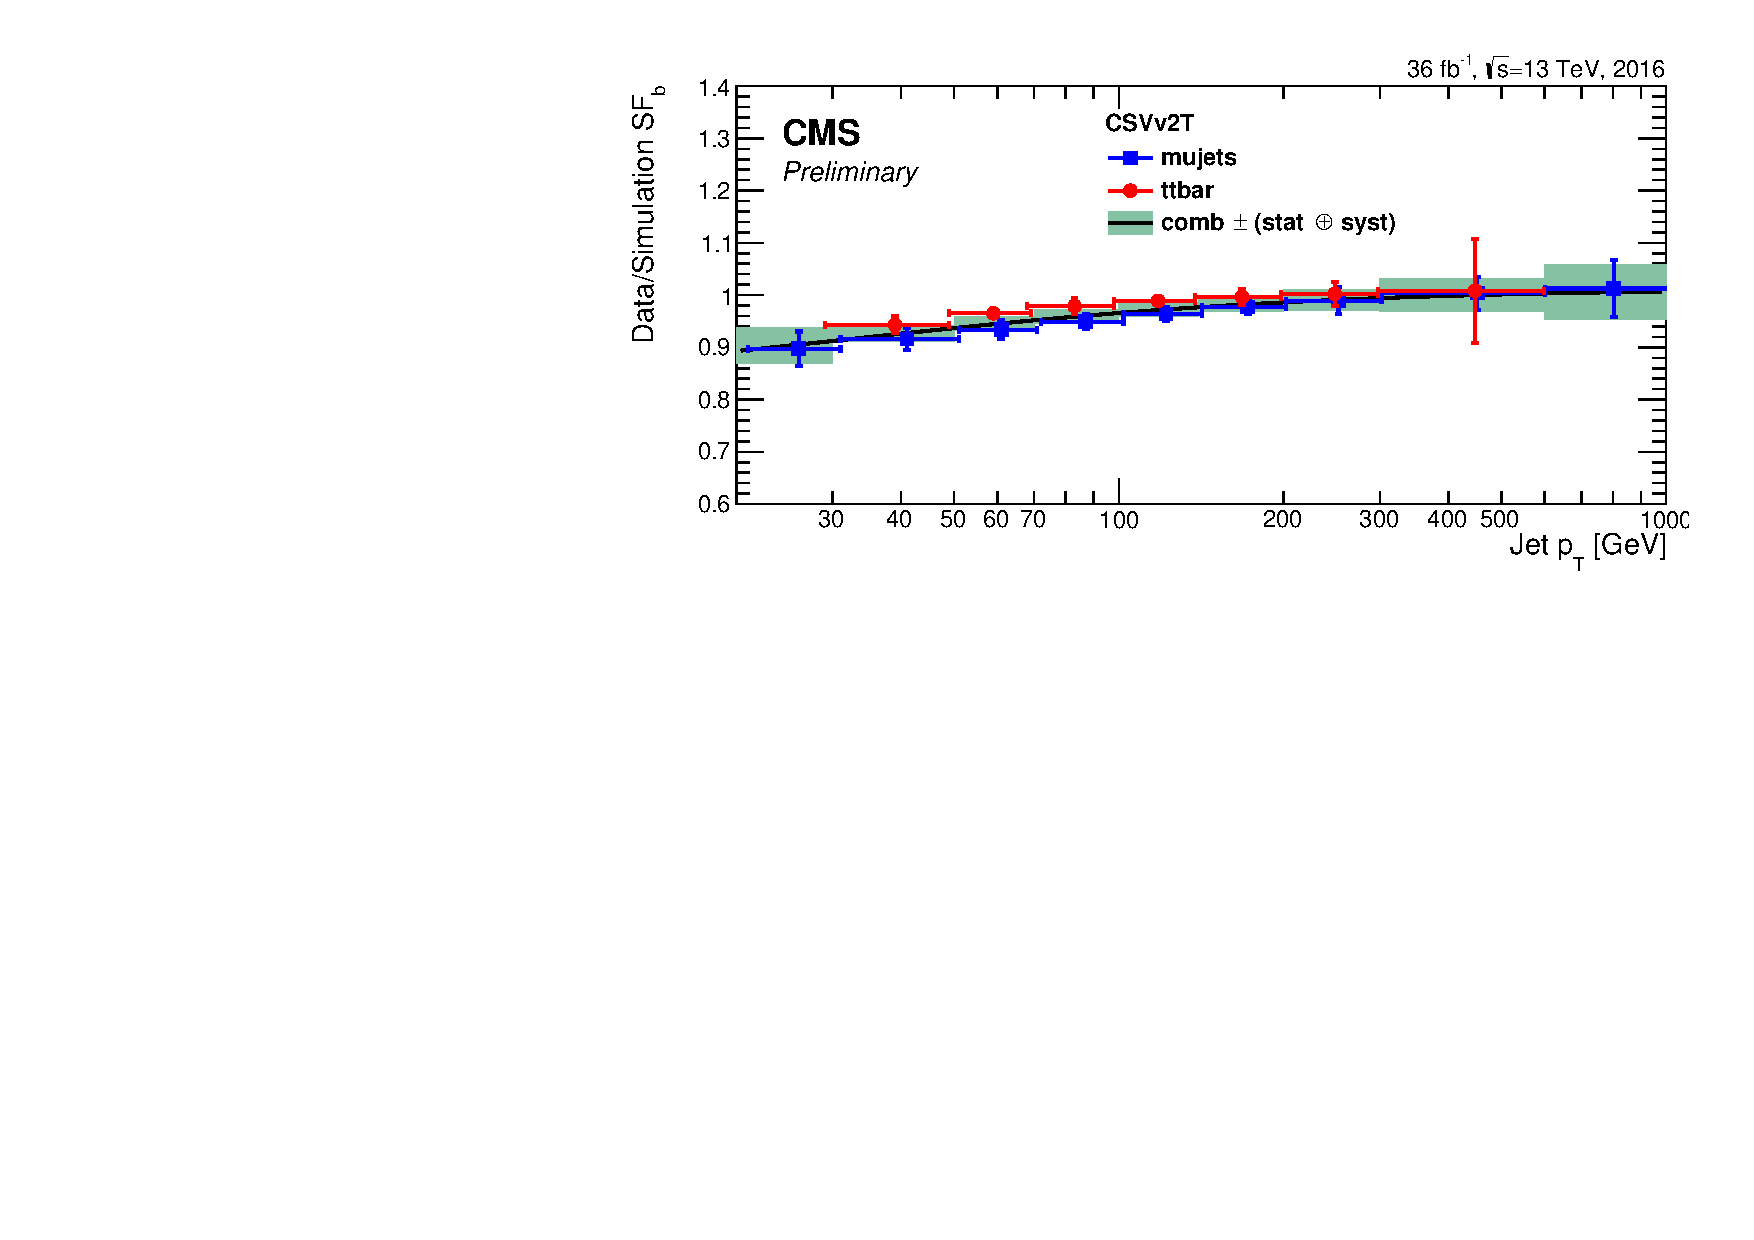
\includegraphics{SimReco/Figures/BTagSF}}  
\caption{Scale factor between the b jet identification efficiency measured in data and simulation. The measurement is performed with events containing jets and muons and in \ttbar events \cite{CMS-DP-2017-012}
  \label{fig:reco_btagsf}}
  \end{center}
\end{figure}

The scale factors are applied to the simulation by reweighting events as follows:

\begin{equation}
w = \frac{P(\mathrm{Data})}{P(\mathrm{MC})} \vspace{0.1cm} P(\mathrm{Data}) = \prod_{i=tagged} \epsilon_i^{data} \prod_{j=not tagged} (1-\epsilon_j^{Data}) \vspace{0.1cm} P(\mathrm{MC}) = \prod_{i=tagged} \mathrm{SF}_i\epsilon_i^{MC} \prod_{j=not tagged} (1-\mathrm{SF}_j\epsilon_j^{MC}).
\end{equation}

Here, the $\epsilon$ denotes the b identification efficiency for a jet for measured data and simulation respectively, while $\mathrm{SF}$ stands for the scale factor for that jet.
Both the efficiency and the scale factor depend on the kinematic properties of the jet.

